\documentclass[11pt]{article}
\usepackage{fullpage}
\usepackage{multirow}
\usepackage{amsmath}
\usepackage{graphicx}
%\usepackage[ruled,vlined]{algorithm2e}
\usepackage[ruled,noline]{algorithm2e}
\usepackage{authblk}

\begin{document}

%%%%%%%%%%%%%%%%%%%%%%
% Title
%%%%%%%%%%%%%%%%%%%%%%
\title{A probabilistic framework for sensitive structural variant discovery}
%\author{Ryan M. Layer$^1$, 
%Gabriel Robins$^1$, 
%Ira M. Hall$^2$,
%and
%Aaron R. Quinlan$^3$\footnote{to whom correspondence should be addressed}}
%
%\address{$^{1}$Department of Computer Science, University of Virginia, Charlottesville, VA\\
%$^{2}$Department of Biochemistry and Molecular Genetics, University of Virginia, Charlottesville, VA\\
%$^{3}$Department of Public Health Sciences and Center for Public Health
%Genomics, University of Virginia, Charlottesville, VA}

\author[1]{Ryan M. Layer}
\author[2]{Ira M. Hall\thanks{\mbox{Corresponding author}}}
\author[2,3]{Aaron R, Quinlan\thanks{\mbox{Corresponding author}}}
\affil[1]{Department of Computer Science, University of Virginia, Charlottesville, VA}
\affil[2]{Department of Biochemistry and Molecular Genetics, University of Virginia, Charlottesville, VA}
\affil[3]{Department of Public Health Sciences and 
Center for Public Health Genomics, University of Virginia, Charlottesville, VA}


\maketitle

%%%%%%%%%%%%%%%%%%%%%%
% Abstract
%%%%%%%%%%%%%%%%%%%%%%
\section{Abstract}
Comprehensive discovery of structural variation (SV) in human genomes from DNA
sequencing requires the integration of multiple alignment ``signals''. However,
owing to inherent technical challenges, most existing SV discovery approaches 
utilize only a single signal. Existing approaches consequently suffer from
low sensitivity, especially at low sequence coverage and for smaller SVs. We
present a novel probabilistic SV discovery framework that is capable of
integrating multiple SV alignment signals. We demonstrate improved sensitivity
over extant methods by combining both paired-end and split-read alignments and
emphasize the utility of our framework for comprehensive studies of structural
variation in often heterogeneous tumor genomes.


%%%%%%%%%%%%%%%%%%%%%%
% Introduction
%%%%%%%%%%%%%%%%%%%%%%
\section{Introduction}

Differences in chromosome structure are a prominent source of natural 
genetic variation in the human population. While such structural variants,
including both balanced (e.g., inversions and reciprocal translocations)
and unbalanced (e.g., deletions and duplications) genomic rearrangements, are 
less common than other forms of genetic variation such as single-nucleotide 
polymorphisms (SNPs), they are typically much larger, and as such, have the 
potential for substantial functional consequence. Spontaneous structural
variants underly many genomic disorders and polymorphic SVs have been shown to
be associated with common diseases \cite{mccarroll2007}. Moreover, extensive
genomic rearrangement is a hallmark of tumor genomes, and complex rearrangements
have been negatively correlated with a tumor's response to chemotherapy
\cite{rausch2012a}.

Our detailed understanding of the landscape of SV in the human genome and the
mechanisms that form them has, in large part, been driven by advances in DNA
sequencing technologies. However, the discovery and genotyping of SV is 
fundamentally more complicated than SNPs; SVs vary both in size and state, 
and SV discovery algorithms must incorporate several distinct alignment 
``signals'' (or a lack thereof) for accurate discovery. Consequently, the
accuracy of existing SV discovery tools remains substantially lower than for
smaller genetic variants. More importantly, most existing SV discovery
tools examine a single type of alignment signal (e.g., either ``split'' or 
``discordant'' alignments). Discovery sensitivity is typically limited as a 
result. The impact of this reduced sensitivity is particularly acute in studying 
cancer, as tumor genomes are often highly heterogeneous, meaning that even 
when cancer genomes are sequenced to high coverage, less frequent rearrangements 
will only be detectable via a small number of sequence alignments. Therefore,
even as the throughput and cost of DNA sequencing continues to improve, the
need for sensitive methods will remain in order to detect evermore rare
genomic events in cancer and in other studies of somatic genome variability.



%%%%%%%%%%%%%%%%%%%%%%
% Results
%%%%%%%%%%%%%%%%%%%%%%
\section{Results}

In this manuscript, we describe a general probabilistic framework for 
integrating diverse SV alignment signals from multiple sources. Our framework is
motivated by the relatively poor sensitivity of SV discovery algorithms
that utilize only one type (e.g., paired-end mapping) of alignment signal.
By providing a flexible framework that can exploit \emph{all} alignment signals,
we seek to improve both discovery sensitivity and specificity and to increase 
the resolution of predicted SV breakpoint regions.

\subsection{Overview of the probabilistic framework}
%1. Walk through the concept (use the high-level figure that Ryan is working on).
%2. What are the signals and the uncertainties associated with them.
%3. How are they integrated?
%4. Describe the quantile/decile cutoff concept.
%5. Describe how this leads to improved sensitivity and resolution.

Our probabilistic framework is based upon a general representation of a SV 
breakpoint that accommodates multiple structural rearrangement signals (for a 
comprehensive review, see \cite{alkan2011}). The use of a generalized framework
allows all SV alignment signals to be integrated into a single discovery
process (Methods). In turn, SV discovery is more sensitivity, 
especially at lower coverage, since many additional SVs may be recovered that 
would otherwise be missed were only a single SV alignment signal considered. 
Similarly, greater specificity can be realized by asserting that, assuming 
reasonable sequence coverage, evidence for true SV should be apparent through 
more than one alignment signal.

We define a breakpoint as a pair of bases that are adjacent in a sample genome 
but not in a reference genome.  To account for the varying level noise inherent 
to different types of alignment evidence (e.g., ``split'' vs. ``discordant'' 
alignments), we represent a breakpoint with pair of probability distributions
spanning the predicted breakpoint regions (Figure 1, Methods).  Each position 
in the two intervals is assigned a probability that represents the relative 
likelihood that the given position represents one end of the breakpoint. 

%Clustering, filtering, and prediction are performed only after all
%signals are mapped to this general representation.  The framework can improve
%prediction sensitive by allowing the detection of variants that do not have
%enough evidence from any one signal to be distinguished from the noise, but do
%have evidence from multiple signals.

Our framework provides distinct modules that map signals from each alignment 
evidence type to our common probability interval pair.  For example, paired-end 
sequence alignments are projected to a pair of intervals upstream or downstream 
(depending on orientation) of the mapped ends (Figure 1).  The size of the 
intervals and the likelihood at each position is based on the size distribution
of the sample's DNA fragment library.  The distinct advantage of this approach
is that \emph{any} type of evidence can be considered, as long there exists
a direct mapping from the alignment signal to breakpoint likelihoods.
Here we provide three modules for converting SV alignment signals to breakpoint
likelihood intervals: paired-end, split-read, and generic.  We emphasize that
our framework is extensible to possible new alignment signals from forthcoming
DNA sequencing technologies \cite{OxfordNanopore}. The paired-end module maps 
the output of a paired-end sequence alignment algorithm 
(e.g., BWA \cite{li2009a}), the split-read module maps the output of a 
split-read sequence alignment algorithm (e.g., YAHA\cite{faust2012}, 
BWA-SW\cite{li2010}), and the generic module allows users to include the result 
SV signal types that do not have specific module implemented (e.g., 
\emph{a priori} knowledge such as known sites of SV, and/or output from 
copy-number variation discovery tools).

Once all of the evidence from the different classes is mapped to breakpoint
intervals, all breakpoints with overlapping intervals are clustered and 
the probability intervals are integrated to refine the evidence for 
rearrangement and the predicted breakpoint interval (see Methods for details).  
Any clustered breakpoint region that contains sufficient evidence (based on 
user-defined arguments) is returned as predicted SV.  
Similar to the breakpoint probability, the clustered probabilities give the 
relative likelihood of a breakpoint.  The resolution of the predicted breakpoint
regions is improved by trimming the positions with probabilities 
in the lower (e.g., the lowest 5 percent) percentile of the distribution.

We have implemented this framework into an open source C++ software package 
(UNNAMED) that is capable of detecting SV from multiple alignment signals in 
BAM alignment file from one or more samples.

\begin{figure}
\center{
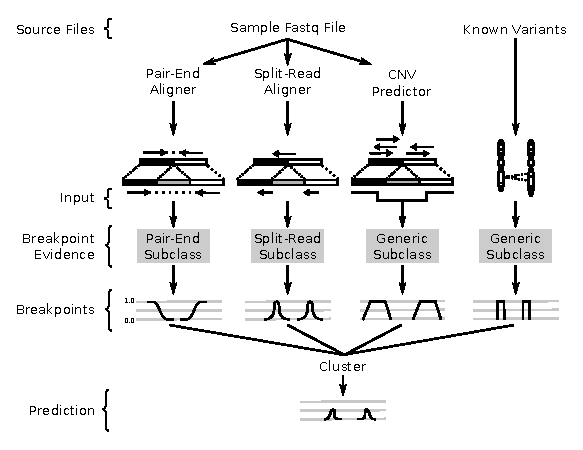
\includegraphics{Workflow.eps}
}
\caption{An example workflow for UNNAMED that uses three different singals
(paired-end, split-read, and read-depth) from one sample, and information about
known variants.}
\label{workflow:fig}
\end{figure}

\subsection{Comparison of discovery performance on simulated datasets}
In order to assess the performance of our framework, we compared our discovery
accuracy using paired-end alignments, split-read alignments, and both signals to 
three widely used SV discovery packages: Hydra \cite{quinlan2010b},
GASVPro \cite{sindi2012} and DELLY \cite{rausch2012b}. We created a simulated 
experimental genome by simulating 1000 deletions, duplications, insertions, 
and inversions (4000 events total) throughout chromosome 10 of the hg19 genome 
using SVsim (Faust et al, \emph{in preparation}).  For each SV event type, half
of the variants were less than 1kb and the other half were greater than 1kb (see
Methods for details).  We used the WGSIM (Heng Li, unpublished) paired-end read 
simulator to \"sequence\" our simulated genome to 2, 5, and 20 fold 
haploid coverage (Methods).

\subsection{Discovery sensitivity}
The predicted SV breakpoints from each discovery approach were compared to the
simulated breakpoints in order to measure each approach's sensitivity (Figure 2) 
and false discovery rate (FDR; Table 1). Not surprisingly, for each approach,
breakpoint discovery sensitivity increases with greater genome coverage.
Moreover, UNNAMED's sensitivity is improved when both paired-end and split-read
alignments are integrated into the probabilistic framework, as compared to 
discovery with either signal alone. In addition, UNNAMED is consistently more
sensitive than other approaches at lower coverage for all SV types. For example,
UNNAMED detects 24.5\% and 79.3\% of all deletions at 2 and 5 fold genome
coverage, whereas HYDRA, the next most sensitive approach, detects 2.9\% and
30.9\%, respectively. 

\begin{figure}
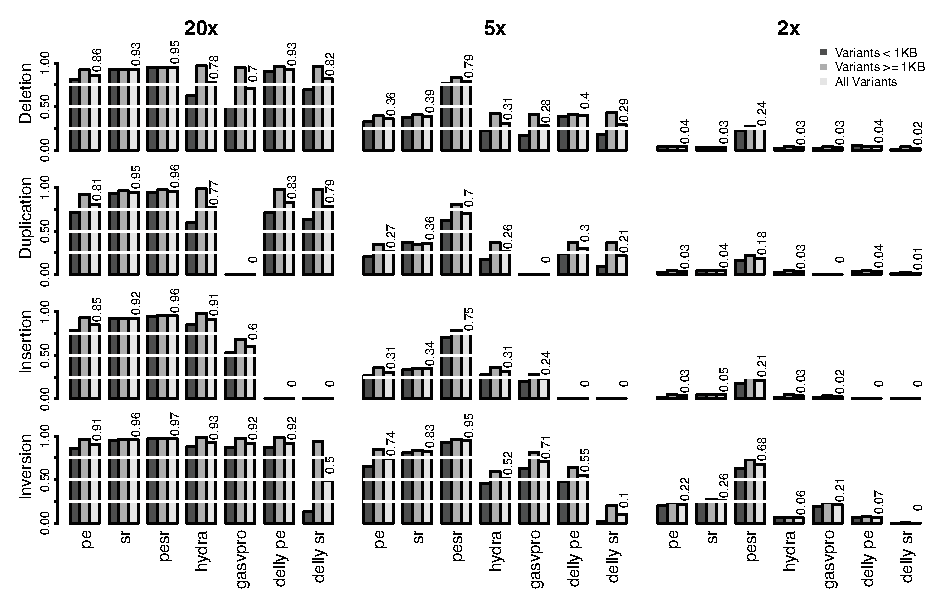
\includegraphics[width=6.5in]{R/ss_sl_s-un_hy_gv_dl-r10x.eps}
\caption{Sensitivity for UNNAMED, Hydra, GASVPro, and Delly.}
\label{sensitivity:fig}
\end{figure}

\textbf{DOUBLE-CHECK ALL OF THE SENSITIVITY NUMBERS BELOW}

At lower coverage (i.e., 2 and 5X), UNNAMED is consistently more sensitive 
than all other approaches across all SV types. At most, UNNAMED was 
8.4 times more sensitive than the second most
sensitive approach at low coverage (UNNAMED 24.5\% vs. HYDRA 2.9\% for deletions
at 2X coverage). At worst, it was 1.2 times more sensitive for inversions at
5X coverage (UNNAMED 96.4\% vs. GASVPRO 80.8\%). At higher (20X) coverage, 
UNNAMED's sensitivity advantage persists; it ranges from 95.6\% to 97.2\% 
across all SV types, whereas HYDRA and GASVPRO range from 76.9\% to 92.8\% and
59.9\% to 91.9\%, respectively (excluding duplications for which GASVPRO is
incapable of making predictions).

Unlike the other tools compared, UNNAMED has nearly equal sensitivity for 
both smaller (i.e. < 1kb) and larger (> 1kb) events. Whereas at 10X coverage,
UNNAMED detects 96.0\% and 95.0\% of deletions less and greater than 1kb, 
respectively, GASVPRO and HYDRA each have much lower sensitivity for small
variants than for large (62.0\% vs 97.0\% for HYDRA and 51.0\% and 95.0\% for
GASVPRO). This increased sensitivity is especially important given that smaller
SVs are much more common than larger events \cite{mills2011}.


\subsection{False discovery rate}
Improved SV discovery sensitivity is crucial for comprehensive characterizations
of the full spectrum of genetic variation in human genomes, yet high
sensitivity at the cost of an inflated false discovery rate (FDR) is
undesirable given the time and cost associated with pursuing the putative 
biological impact of spurious variation.

We compared the FDR for each SV discovery tool using the same simulated
SVs as described above (Table 1).The false discovery rate for all tools ranged 
from 0.0\% to 24.2\%. Overall, DELLY-SR had the lowest FDR across all SV types
and genome coverage levels, yet the conservative calling comes at the cost of
lower sensitivity compared to the other tools. While UNNAMED's FDR was 
slightly higher than GASVPRO for deletions, its FDR was consistently 
low (0.0\% - 5.0\%) across all SV types and coverage levels. In contrast, 
GASVPRO had much higher FDRs for insertions and inversions and
its FDR increased at lower coverage levels.  HYDRA had consistent FDRs across
SV types and coverage levels (0.0\% to 8.9\%), yet these rates were always 
higher than the analogous UNNAMED FDRs. These results indicate that UNNAMED's
probabilistic framework afford substantial improvements in discovery
sensitivity while maintaining low false discovery rates.

%\begin{table}[h!b!p!]
%\caption{False discovery rates for each SV discovery approach.}
%\begin{tabular}{l|llll}
%			& 20x			& 10x			& 5x			& 2x \\
%\cline{2-5}
%			& \multicolumn{4}{c}{Deletions} \\
%\cline{1-5}
%pe		&	0.014	&0.009	&0.008	&0 \\
%sr      &    0.006	&0.001	&0		&0 \\
%pesr    &    0.018	&0.007	&0.005	&0 \\
%hydra   &    0.038	&0.01	&0.006	&0 \\
%gasvpro &    0		&0		&0		&0 \\
%delly pe&    0.002	&0.001	&0		&0 \\
%delly sr&    0		&0		&0		&0 \\
%\cline{2-5}
%			& \multicolumn{4}{c}{Duplications} \\
%\cline{2-5}
%
%pe          &0.004	&0.003	&0		&0 \\
%sr          &0.005	&0.002	&0.003	&0 \\
%pesr        &0.007	&0.005	&0.001	&0 \\
%hydra       &0.03	&0.006	&0.011	&0 \\
%gasvpro     &N/A	&	N/A	&	N/A	&	N/A	 \\
%delly pe    &0		&0		&0		&0.028 \\
%delly sr    &0		&0		&0		&0 \\
%\cline{2-5}
%			& \multicolumn{4}{c}{Insertions} \\
%\cline{2-5}
%
%pe          &0.042	&0.02	&0.016	&0 \\
%sr          &0.013	&0.002	&0.006	&0 \\
%pesr        &0.05	&0.018	&0.009	&0 \\
%hydra       &0.089	&0.034	&0.034	&0.03 \\
%gasvpro     &0.242	&0.131	&0.065	&0.041 \\
%delly pe    &N/A		&N/A		&N/A		&N/A \\
%delly sr    &N/A		&N/A		&N/A		&N/A \\
%\cline{2-5}
%			& \multicolumn{4}{c}{Inversions} \\
%\cline{2-5}
%
%pe          &0.004	&0		&0		&0 \\
%sr          &0.004	&0.002	&0.001	&0 \\
%pesr        &0.009	&0.002	&0.002	&0 \\
%hydra       &0.054	&0.013	&0.006	&0 \\
%gasvpro     &0.005	&0.032	&0.082	&0.079 \\
%delly pe    &0		&0		&0		&0 \\
%delly sr	&0.004	&0		&0		&0 \\
%\end{tabular}
%\end{table}


\begin{table}[h!b!p!]
\small
\caption{False discovery rates for each SV discovery approach.}
\begin{tabular}{l|lll|lll|lll|lll}
		Coverage
		&20x&5x&2x &20x&5x&2x &20x&5x&2x &20x&5x&2x \\
\cline{1-13}
			Variety
			&\multicolumn{3}{c}{Deletions} 
			&\multicolumn{3}{|c}{Duplications} 
			&\multicolumn{3}{|c}{Insertions}
			&\multicolumn{3}{|c}{Inversions} \\
\cline{1-13}
pe		&0.014&0.008&0&0.004&0	  &0    &0.042&0.016&0	  &0.004&0	  &0 \\
sr      &0.006&0	&0&0.005&0.003&0	&0.013&0.006&0	  &0.004&0.001&0 \\
pesr    &0.018&0.005&0&0.007&0.001&0	&0.05 &0.009&0	  &0.009&0.002&0 \\
hydra   &0.038&0.006&0&0.03 &0.011&0	&0.089&0.034&0.03 &0.054&0.006&0 \\
gasvpro &0	  &0	&0&N/A  &N/A  &N/A  &0.242&0.065&0.041&0.005&0.082&0.079 \\
delly pe&0.002&0	&0&0	&0	  &0.028&N/A  &N/A	&N/A  &0	&0	  &0 \\
delly sr&0	  &0	&0&0	&0	  &0	&N/A  &N/A	&N/A  &0.004&0	  &0 \\ 

\end{tabular}
\label{table:fdr}
\end{table}


\subsection{Increased breakpoint resolution}
By integrating both paired-end and split-read SV signals, the resolution of
our predicted breakpoint intervals is increased relative to the resolution 
yielded by examining either signal on its own (Figure~\ref{resolution:fig}). The biggest increase
in resolution comes from split-read alignments, as, in principle, split-reads
map SV breakpoints to a single base pair. In practice, however, there is
often local alignment ambiguity at the breakpoint which reduces breakpoint 
resolution to 2-5bp \cite{quinlan2010b}. Therefore, in order to capture all
split-reads supporting a given breakpoint, we examine a ``window'' surrounding
a putative breakpoint (e.g. +/- 20bp). This allows greater \emph{discovery}
sensitivity (i.e., more alignments are included) at the cost of slightly reduced
breakpoint \emph{resolution}. Consequently, at 2X coverage, our combined
deletion breakpoint resolution is 42bp. However, at 20X coverage, our resolution
increases to 5bp \textbf{ARQ: I still don't entirely understand the jump from
42bp to 5bp at 5x versus 20x.  Seems odd.}. Importantly, the breakpoint 
resolution for all other SV types were nearly identical to resolution for 
deletions (data not shown).


\begin{figure}
\center{
\includegraphics[width=2.5in]{R/resolution-un.eps}
}
\caption{Breakpoint resolution measured as the median interval size in bp for
true positive deletion calls at 20x, 5x, and 2x coverage.}
\label{resolution:fig}
\end{figure}



\subsection{Benchmarks using 1000 Genomes datasets}
\textbf{Speed with 1, 2, 3, ..., 10 samples.  How many events per sample?
Need to use both PE and SR.}
To assess the utility of our framework for SV discovery in typical human genome
sequencing datasets, we combined whole-genome alignment signals from between 1 
and 10 samples from the 1000 Genomes Project \cite{durbin2010}. The runtimes
of our software ranged from X to Y minutes when exploring alignments from 1 and
10 samples, respectively, and the maximal memory usage was Z, indicating that
our framework provides improved SV discovery in reasonable time-frames using
resources that are available in typical research computing environments. When
combining alignments from all 10 samples, the median number of predicted SV
breakpoints per sample was X, which is well in the range of SV 
breakpoints for a typical human genome \cite{mills2011}.


%%%%%%%%%%%%%%%%%%%%%%
% Discussion
%%%%%%%%%%%%%%%%%%%%%%
\section{Discussion}
We have developed a general probabilistic framework for accurate SV discovery, 
and we have demonstrated that our framework is more sensitive than existing 
discovery tools across all SV types and coverage levels. Importantly, the
increased sensitivity does not come at the cost of excessive spurious SV
predictions. While our FDR was slightly higher for deletions than other tools,
we note that the integration of third-party copy-number predictions into
our calling framework (using the generic module, Figure 1) would bring our 
deletion FDR to nearly zero.

Given the increased sensitivity, efficiency, and ease of use of our framework, 
we emphasize its utility for comprehensive SV discovery in human genomes. 
Increased sensitivity is especially important for cancer studies, as tumors are 
often comprised of highly heterogeneous genomes. As we demonstrate clearly
superior sensitivity at low coverage (which is a proxy for low frequency 
rearrangements), we argue that our framework well-suited to detailed studies
	of tumor heterogeneity and somatic genome variability.\\




% Points to make:\\
% 1. Mention that the framework is extensible to multiple samples. \\
% 2. Mention that we presented results for PE and SR, but it can be 
% improved by integrating CN, existing calls, etc.  Even though our FDR for 
% deletions is already quite low, we anticipate that it could be brought to ~0
% by integrating CN calls from another tool.\\
% 3. The simulation is whole-genome unlike simulations done by other tools, 
% and as such, we feel that the results have a stronger grounding in reality
% than others.\\
% 4. The tool is easy to use, runs in reasonable times, and produces highly
% sensitive and specific results.\\
% 5. Utility for cancer and studies of somatic instability, etc.\\



%%%%%%%%%%%%%%%%%%%%%%
% Methods
%%%%%%%%%%%%%%%%%%%%%%
\section{Methods}

We propose a breakpoint prediction framework that can accommodate multiple
classes of evidence from multiple sources in the same analysis.  To accomplish
this, we define a high-level breakpoint type that represents the consensus
breakpoint location from different pieces of evidence.  Our framework makes use
of an abstract breakpoint evidence type to define a set of functions that serve
as an interface between specific evidence subtypes (e.g., paired-end sequence
alignments and split-read mappings) and the breakpoint type.  Any class of
evidence for which these functions can be defined may be included in our
framework.  To demonstrate the applicability of this abstraction, we defined
three breakpoint evidence subtypes: paired end sequencing, split read mapping,
and a general breakpoint interface. 

Since our framework combines evidence from multiple classes, it extends
naturally to include evidence from multiple sources.  The sources that can be
considered in a single analysis may be any combination of evidence from
different samples, different evidence subclasses from the same samples, or
data sets from known genomic features.  We refer to a given data set as a
breakpoint evidence instance, and assume that each instance contains only one
evidence subtype and is from a single sample.  To help organize the results of
analysis with multiple samples or multiple instances for a single sample,
each instance is assigned an id that can be shared across instances.


\subsection{Breakpoint}

A breakpoint is a pair of genomic sequences that are adjacent in a sample genome
but not in a reference genome. Breakpoints can be detected, and their locations
predicted by various evidence classes (e.g., paired-end sequence alignments and
split-read mappings).  To support the inclusion of different evidence classes
into a single analysis, we define a high-level breakpoint type as a collection
of the evidence that corroborates the location and variety of a particular
breakpoint.  Since many evidence classes provide a range of possible breakpoint
locations, we represent the breakpoint's location with a pair of breakpoint
intervals where each interval has a a start position, an end position, and a
probability array that represents the likelihood that a given position in the
interval is one end of the breakpoint.  More formally, a breakpoint is a tuple 
$b=\langle E,l,r,v \rangle$ where
\begin{itemize}
\item $E$ is the set of evidence that corroborates the location and variety of a
particular breakpoint
\item $l$ and $r$ are left and right breakpoint intervals each with values
	$\langle s, e, p \rangle$ where
	\begin{itemize}
		\item $s$ and $e$ are the start and end genomic coordinates
		\item $p$ is a probability array where $|p|=e-s$ and $p[i]$ is the
		relative probability that position $s+i$ is one end of the breakpoint
	\end{itemize}
%\item $w=\sum\limits_{i=1}^{|E|} E_i.w $ cumulative breakpoint weight, were
%each evidence weight represents the level of confidence in the associated
%instance 
\item  $v$ is the breakpoint variety (e.g., $\textsc{Deletion}$,
$\textsc{Duplication}$, etc.)
\end{itemize}

If there exits two breakpoints $b$ and $c$ in the set of all breakpoints $B$
where $b$ and $c$  intersect ($b.r$ intersects $c.r$, $b.l$ intersects $c.r$,
and $b.v = c.v$), then $b$ and $c$ are {\em merged} into interval $m$, $b$ and
$c$ are removed from $B$, and $m$ is placed into $B$.  The merged breakpoint $m$ is defined as $\langle E = b.E + c.E, l_n, r_n, v = b.v = c.v\rangle$, where 
$l_n.s = \max(b.l.s, c.l.s)$, $l_n.e = \min(b.l.e, c.l.e)$, similar for $r_n$.
Once all evidence has been considered, the breakpoints in $B$ are enumerated.
Since each genomic interval has a probability array associated with it, the
intervals may be trimmed to include only the positions that meet are in the top
percentile (e.g., top 99.9 percent of values).

\subsection{Breakpoint Evidence}

To link the specifics of data like paired end sequencing alignments and split
read mappings to the general breakpoint type defined above, we define an
abstract breakpoint evidence type.  This abstract type defines an interface that
allows for the inclusion of any data that can provide the following functions:

\begin{itemize}
	\item $\textsc{is\_bp}$ determines if a particular
	instance of the data contains evidence of a break point
	\item $\textsc{get\_v}$ determines the breakpoint 
	variety (e.g., deletion, duplication, inversion, etc.)
	\item $\textsc{get\_bpi}$ maps the data to a pair of
	breakpoint intervals
	%\item $\textsc{get\_w()}$ that represents the level of confidence
	%that a specific data type is evidence of a real breakpoint
\end{itemize}

To demonstrate the applicability of this abstraction, we defined three
breakpoint evidence instances: paired end sequencing alignments, split read
mapping, and a general breakpoint interface.  Paired end sequencing and split
read mapping are among the most frequently used data types for breakpoint
detection, and the general interface provides a mechanism to include any other
breakpoint information such as known breakpoints or output from other analysis
pipelines.  As technologies evolve and our understanding of structural
variations improves, other instances can be easily added.

\subsubsection{Paired End Sequencing Alignments}

Paired end sequencing involves fragmenting genomic DNA into roughly uniformly
sized segments, and sequencing both ends of each segment to produce the sequence
pair $\langle x,y \rangle$.  The ends of the pair are
aligned to a reference genome $R(x)=<o,s,e>$, where $o=+|-$ indicates the
alignment orientation, and $s$ and $e$ delineate the start and end positions of
the matching sequence in the reference genome.  To simply the explanation, we
let the genome be one contiguous interval of concatenated chromosomes so that
all sequences can be referred to by offset only.  Translocations can still be
identified in this model since the positions on different chromosomes will be
far apart.  We also assume that both $x$ and $y$ align uniquely to the
reference and that $R(x).s<R(x).e<R(y).s<R(y).e$.  While it is often not
possible find the exact position of a sequence in the sample genome, it is
useful to refer to $S(x)=<o,s,e>$ as the alignment of $x$ with respect to the
originating sample's genome.  

% is_bp
Assuming the reads were made on an Illumina platform, pairs are expected to
align to the reference genome with a $R(x).o=+, R(y).o=-$ orientation, and at
distance $R(y).e - R(x).s$ roughly equivalent to the fragmentation length from
the sample preparation step.  Any pair that aligns with an unexpected
configuration can be evidence of a breakpoint.  These unexpected configurations
include matching orientation $R(x).o = R(y).o$, alignments with switched
orientation $R(x).o=-, R(y).o=+$, and an apparent fragment length ($R(y).e -
R(x).s$) that is either shorter or longer than expected.  We estimated the
expected fragment length to be the sample mean $\overline{l}$ fragment length,
and the fragment length standard deviation to be the sample standard deviation
$\overline{s}$ from the set of properly mapped pairs (as defined by the SAM
spec) in the sample data set.  Considering the variability in the sequencing
process, we extend the expected fragment length to include sizes 
$\overline{l}\pm v_l \overline{s}$, where $v_l$ is a tuning parameter that
reflects spread in the data.

%\begin{algorithm}[H]
%    \DontPrintSemicolon
%    \footnotesize
%	\KwIn{Reference genome $R$, 
%		  Sequence pairs $\langle x,y \rangle$,
%		  expected fragment length $\overline{l}$ 
%			and standard deviation $\overline{s}$,
%		  tuning parameter $d$ }
%    \KwOut{$\textsc{true}$ if $\langle x,y \rangle$ have an unexpected
%		   alignment, otherwise $\textsc{false}$}
%    \BlankLine
%    \textbf{Function} $\textsc{is\_bp}$\;
%	\Begin{
%		\uIf{$R(x).s = R(y).s$}
%			{\Return \textsc{true}\;}
%		\uElseIf{$ R(y).e - R(x).s > \overline{l} + z*\overline{s}$}
%			{\Return \textsc{true}\;}
%		\uElseIf{$ R(y).e - R(x).s < \overline{l} - z*\overline{s}$}
%			{\Return \textsc{true}\;}
%		\uElse
%			{\Return \textsc{false}\;}
%	}
%	\caption{Breakpoint evidence function that determines if a paired end
%			 sequencing alignment contains evidence of a break point.}
%    \label{is_bp}
%\end{algorithm}

% get_v
% +- deletion or insertion
% ++ inversion
% -+ duplication
% -- inversion
The breakpoint variety for $\langle x,y \rangle$ can be inferred from the 
orientation that $x$ and $y$ align to in the reference.  If the orientations
match, then the breakpoint was caused by an inversion event, and if the
$R(x).o=-$ and $R(y).o=+$ then there was a duplication event.  When $R(x).o=+$
and $R(y).o=-$, the breakpoint variety is ambiguous between an insertion and a
deletion.  This ambiguity is also true for other types of evidence types (e.g.,
split read mappings).  While it may be possible to determine which event caused
the breakpoint in a post-processing step, breakpoint correlation is a complex
process and is beyond the scope of this framework.  Since we cannot distinguish
between the two varieties, any pair with a $+/-$ orientation configuration is
marked as a deletion.  
%Given $R(x).o$ and $R(y).o$, we can define the
%function $\textsc{get\_v()}$ for the paired end sequence alignment
%data type in Algorithm~\ref{get_v}.

%\begin{algorithm}[H]
%    \DontPrintSemicolon
%    \footnotesize
%	\KwIn{Reference genome $R$, 
%		  Sequence pairs $\langle x,y \rangle$}
%    \KwOut{Breakpoint variety for $\langle x,y \rangle$}
%    \BlankLine
%    \textbf{Function} $\textsc{get\_v}$\;
%    %\textbf{Function} $\textsc{get\_v}(R(x).o,R(y).o)$\;
%	\Begin{
%		\uIf{$R(x).o = R(y).o$}
%			{\Return \textsc{Inversion}\;}
%		\uElseIf{$R(x).o = - \textbf{ and } R(y).o = +$}
%			{\Return \textsc{Duplication}\;}
%		\uElseIf{$R(x).o = + \textbf{ and } R(y).o = -$}
%			{\Return \textsc{Deletion}\;}
%	}
%	\caption{Breakpoint evidence function that determines the breakpoint variety
%			 for paired end sequencing alignments.}
%    \label{get_v}
%\end{algorithm}

% get_bpi
To map $\langle x,y \rangle$ to breakpoint intervals $l$ and $r$, the ranges of
possible breakpoint locations must be determined and probabilities assigned to
each position in those ranges.  By convention, $x$ maps to $l$ and $y$ to
$r$, and for the sake of brevity we will focus on $x$ and $l$ since the same
process applies to $y$ and $r$.  Assuming that a single breakpoint exists
between $x$ and $y$, then the sign of $x$ determines if $l$ will be upstream
or downstream of $x$.  If the $R(x).s=+$, then the breakpoint interval begins
after $R(x).e$ (downstream), otherwise the interval ends before $R(x).s$
(upstream).  
%To account for variance in the alignment of $x$, we extend the breakpoint by
%to $R(x).e - v_a$ if $R(x).s=+$ and $R(x).s + v_a$ if $R(x).s=-$,
%where $v_a$ is a turning parameter.

The length of each breakpoint interval is proportional to the expected fragment
length $\overline{l}$ and standard deviation $\overline{s}$.  Since we assume
that only one breakpoint exists is between $x$ and $y$, and that it is unlikely
that the distance between the ends of a pair in the sample genome ($S(y).e -
S(x).s$) is greater than $\overline{l}$, then it is also unlikely that one end
of the breakpoint is at a position greater than $R(x).s + \overline{l}$,
assuming that $R(x).o=+$. If $R(x).o=-$, then it is unlikely that a breakpoint
is at a position less than $R(x).e - \overline{l}$.  To account for variability
in the fragmentation process, we extend the breakpoint to 
$R(x).e + (\overline{l} + v_f\overline{s})$ when $R(x).o=+$, and 
$R(x).s - (\overline{l} + v_f\overline{s})$ when $R(x).o=-$, 
where $v_f$ is a tuning parameter that, like $v_l$, reflects the spread in the
data.

The probability that a particular position $i$ in the breakpoint interval $l$ is
part of the actual breakpoint can be estimated by the probability that $x$ and
$y$ span that position in the sample. For $x$ and $y$ to span $i$, the fragment
that produced $\langle x,y \rangle$ must be longer than then distance from the
start of $x$ to $i$, otherwise $y$ would occur before $i$ and $x$ and$y$ would
not span $i$ (contradiction).  The resulting probability is 
$P(S(y).e - S(x).s > i - R(x).s)$ if $R(x).o=+$, and 
$P(S(y).e - S(x).s > R(x).e - i)$ if $R(x).o=-$.
While we cannot directly measure the sample fragment length ($S(y).e - S(x).s$),
we can estimate its distribution by constructing a frequency-based cumulative
distribution $D$ of fragment lengths from the same sample that was used to find
$\overline{l}$ and $\overline{s}$, where $D(j)$ gives the proportion of the
sample with fragment length greater than $j$(Algorithm~\ref{get_one_bpi} and
Algorithm~\label{get_bpi}).

\begin{algorithm}[H]
    \DontPrintSemicolon
    \footnotesize
	\KwIn{Reference genome $R$, 
		  One end of a sequence pair $z$,
		  expected fragment length $\overline{l}$ 
		  and standard deviation $\overline{s}$,
		  tuning parameter $v_f$,
		  fragment length cumulative distribution $D$}
    \KwOut{One end of a breakpoint interval $t$}
    \BlankLine
    \textbf{Function} $\textsc{get\_one\_bpi}$\;
		%$\textsc{get\_one\_bpi}(R,z,\overline{l},\overline{s},v_f,D)$\;
	\Begin{
		\uIf{$R(x).o = +$} {
			$t.s \gets R(z).e$\;
			$t.e \gets R(z).e + \overline{l} + v_f*\overline{s}$\;
			\For{$i = 1 \to ( t.e - t.s ) $} {
				$t.p[i] \gets D(j)$\;
			}
		}
		\uElse {
			$t.e \gets R(z).s$\;
			$t.s \gets R(z).s - (\overline{l} + v_f*\overline{s})$\;
			\For{$i = 1 \to ( l.e - l.s ) $} {
				$t.p[(t.e-t.s) - i] \gets D(j)$\;
			}
		}	
		\Return $t$\;
	}
	\caption{Breakpoint evidence function that maps one end of a sequence pair
			to one end of a breakpoint interval.}
    \label{get_one_bpi}
\end{algorithm}

\begin{algorithm}[H]
    \DontPrintSemicolon
    \footnotesize
	\KwIn{Reference genome $R$, 
		  Sequence pair $\langle x,y \rangle$,
		  expected fragment length $\overline{l}$ 
		  and standard deviation $\overline{s}$,
		  tuning parameter $v_f$,
		  fragment length cumulative distribution $D$}
   \KwOut{Breakpoint intervals $l$ and $r$}
    \BlankLine
    \textbf{Function} $\textsc{get\_bpi}$\;
		%(R,\langle x,y \rangle,\overline{l},\overline{s},v_f,D)$\;
	\Begin{
		$l \gets \textsc{get\_one\_bpi}(R,x,\overline{l},\overline{s},v_f,D)$\;
		$r \gets \textsc{get\_one\_bpi}(R,y,\overline{l},\overline{s},v_f,D)$\;
		\Return $l,r$
	}
	\caption{Breakpoint evidence function that maps a sequence pair alignment to
			a breakpoint interval.}
    \label{get_bpi}
\end{algorithm}

% get_w

%The weight of each sequence pair is an input parameter $v_w$.

\subsubsection{Split Read Alignments}

A split read alignment is a single DNA fragment $X$ that does not uniquely align
to the reference genome, but contains a contiguous ordered set of substrings
$(x_1, x_2, \dots, x_n)$ where $X=x_1x_2\dots x_n$, each substring aligns
uniquely to the reference $R(x_i)=\langle o,s,e \rangle$, and adjacent
substrings align to non-adjacent location in the reference genome
$R(x_{i}).e \neq R(x_{i+1}).s + 1$ for $1\leq i \leq n-1$. A single split read
alignment maps to a set of adjacent split-read sequence pairs 
$(\langle x_1 , x_2 \rangle, \langle x_2, x_3 \rangle, \dots ,
\langle x_{n-1},x_n \rangle)$, and each pair $\langle x_i,x_{i+1} \rangle$ is
considered individually.

% is_bp
By definition, a split-read mapping is evidence of a breakpoint and therefore
the function $\textsc{is\_bp}$ trivially returns $\textsc{true}$.

% get_v
Both orientation and mapping location must be considered to infer the breakpoint
variety for $\langle x_i,x_{i+1} \rangle$.  When the orientations match
$R(x_{i}).o=R(x_{i+1}).o$, the event was either a deletion or
a duplication.  Assuming the $R(x_{i}).o=R(x_{i+1}).o=+$, 
$R(x_{i}).s<R(x_{i+1}).s$ indicates a gap caused by a deletion and 
$R(x_{i}).s>R(x_{i+1}).s$ indicated a repeated sequenced caused by a
duplication.   These observations are flipped when orientations
$R(x_{i}).o=R(x_{i+1}).o=-$.  Similar to paired end alignments, we do not mark
breakpoints as insertions since we cannot distinguish between deletions
and insertions.  When the orientations do not match $R(x_{i}).o \ne
R(x_{i+1}).o$, the event was an inversion and the mapping locations do not need
to be considered.
% Given $R(x_i).o$, $R(x_i).s$, $R(x_{i+1}).o$, and $R(x_{i+1}).s$,
%we can define the function $\textsc{get\_v()}$ for the paired end sequence
%alignment data type in Algorithm~\ref{get_v_sr}.
%
%\begin{algorithm}[H]
%    \DontPrintSemicolon
%    \footnotesize
%	\KwIn{Reference genome $R$, 
%		  Sequence pairs $\langle x,y \rangle$}
%    \KwOut{Breakpoint variety for $\langle x,y \rangle$}
%    \BlankLine
%    \textbf{Function} $\textsc{get\_v}$\;
%	\Begin{
%		\uIf{$R(x_i).o \ne R(x_{i+1}).o$}
%			{\Return \textsc{Inversion}\;}
%		\uElseIf{$R(x_i).o=R(x_{i+1}).o=+ \textbf{ and } R(x_i).s<R(x_{i+1}).s$}
%			{\Return \textsc{Deletion}\;}
%		\uElseIf{$R(x_i).o=R(x_{i+1}).o=- \textbf{ and } R(x_i).s>R(x_{i+1}).s$}
%			{\Return \textsc{Deletion}\;}
%		\uElseIf{$R(x_i).o=R(x_{i+1}).o=+ \textbf{ and } R(x_i).s>R(x_{i+1}).s$}
%			{\Return \textsc{Duplication}\;}
%		\uElseIf{$R(x_i).o=R(x_{i+1}).o=- \textbf{ and } R(x_i).s<R(x_{i+1}).s$}
%			{\Return \textsc{Duplication}\;}
%	}
%	\caption{Breakpoint evidence function that determines the breakpoint variety
%			 for split-read alignments.}
%    \label{get_v_sr}
%\end{algorithm}

% get_bpi
The possibility of errors in the sequencing and alignment processes create some
ambiguity in the exact location of the breakpoint associated with a split-read
sequence pair.  To account for this, each pair $\langle x_i, x_{i+1} \rangle$
maps to two breakpoint intervals $l$ and $r$ centered at the split. The 
probability vectors $l.p$ and $r.p$ are highest at the midpoint and
exponentially decreasing toward their edges.  The size of this interval is a
configurable parameter $v_s$ and is based on the quality of the sample under
consideration and the specificity of the alignment algorithm used to map the
sequences to the reference.

Depending the breakpoint variety, the intervals $l$ and $r$ are centered on
either the start or the end of $R(x_i)$ and $R(x_{i+1})$.  When the breakpoint
is a deletion $l$ is centered at $R(x_i).e$ and $r$ at $R(x_{i+1}).s$, and when
the breakpoint is a duplication $l$ is centered at $R(x_i).s$ and $r$ at
$R(x_{i+1}).e$.  If the breakpoint is an inversion, $l$ and $r$ are both 
centered either at the start positions or end positions of $R(x_i)$ and
$R(x_{i+1})$, respectively.  Assuming that $R(x_i).s<R(x_{i+1}).s$, if
$R(x_i).o=+$ then $l$ and $r$ are centered at $R(x_i).e$ and  $R(x_{i+1}).e$,
otherwise they are centered at $R(x_i).s$ and  $R(x_{i+1}).s$.  If
$R(x_i).s>R(x_{i+1}).s$, then the conditions are swapped.


\begin{algorithm}[H]
    \DontPrintSemicolon
    \footnotesize
	\KwIn{Reference genome $R$, 
		  Split-read pair $\langle x_i,x_{i+1} \rangle$,
		  tuning parameter $v_s$,
		  breakpoint variety $v$ }
   \KwOut{Breakpoint intervals $l$ and $r$}
    \BlankLine
    \textbf{Function} $\textsc{get\_bpi}$\;
	\Begin{
		$l_c \gets NULL$	
		$r_c \gets NULL$	

		\uIf{$v = \textsc{Inversion}$} {

			\uIf{$R(x_i).s<R(x_{i+1}).s$} {
				\lIf{$R(x_i).o=+$}
					{$l_c\gets R(x_i).e,r_c\gets R(x_{i+1}).e$}\;
				\lElse {$l_c\gets R(x_i).s,r_c\gets R(x_{i+1}).s$}\;
			} \Else {
				\lIf{$R(x_i).o=+$}
					{$l_c\gets R(x_i).s,r_c\gets R(x_{i+1}).s$}\;
				\lElse
					{$l_c\gets R(x_i).e,r_c\gets R(x_{i+1}).e$}\;
			}

		}
		\lElseIf{$v = \textsc{Deletion}$} 
			{$l_c\gets R(x_i).e,r_c\gets R(x_{i+1}).s$}\;
		\lElseIf{$v = \textsc{Duplication}$} 
			{$l_c\gets R(x_i).s,r_c\gets R(x_{i+1}).e$}\;

		$l.s\gets l_c - v_s, l.e\gets l_c + v_s$\;
		$r.s\gets r_c - v_s, r.e\gets r_c + v_s$\;

		$\lambda = \log(1e-10)/-v_s$\;
		\For{$i = 1 \to v_s $} {
			$l.p[i] \gets r.p[i] \gets \exp^{-\lambda(v_s - i)}$
		}
		\For{$i = v_s \to 2*v_s $} {
			$l.p[i] \gets r.p[i] \gets \exp^{-\lambda(i - v_s)}$
		}
	
		\Return $l,r$
	}
	\caption{Breakpoint evidence function that maps a sequence pair alignment to
			a breakpoint interval.}
    \label{get_bp_sr}
\end{algorithm}

% get_w

%The weight of each sequence pair is an input parameter $v_w$.

\subsubsection{Generic Evidence}

The generic evidence subclass provides a mechanism to include a wide variety of
data, from known variants to tool output.

two example, known variants and CNV

\subsubsection{Simulation}

Simulated data was used to compare the sensitivity and false discovery rate of
UNNAMED to other SV detection algorithms that rely on either a single signal
(Hydra and DELLY PE) or multiple signals (GASVPro and DELLY SR).  The seed
sequence for all simulations was chromosome 10 from the human reference genome
(hg19).  For each SV variety considered (deletions, duplications, insertions,
and inversions), we used SVsim [XX] to simulate a new version of the seed that
contained 1000 randomly placed, non-overlapping variants ranging between 100 bp
and 10000 bp. Next, wgsim [XX] was used to sample pair-end reads with a 150bp
read length, 500 bp mean outer distance with a 50 bp standard deviation, and
default error rate settings.  Each simulated genome was sampled to 20x, 5x, and
2x coverage. Paired-end reads were mapped to the seed sequence with BWA using
default parameters.  From the BWA output, all split-reads and unmapped reads
were realigned with the split-read aligner YAHA using a word length of 11 and a
minimum match of 15. The TWA output was used as input to UNNAMED PE
(paired-end), Hydra, DELLY (both versions) and GASVPro, the YAHA output was used
as input to UNNAMED SR (split-read), and both BWA and YAHA output were used as
input to UNNAMED PESR (paired-end and split-read).  In all algorithms, the
minimum evidence threshold was four.  For UNNAMED, the turning parameters $v_l$
and $v_f$ were set to four, and alignments with mapping qualities equal to zero
were not considered.

The reads predicted by each algorithm were compared to the events produced by
SVsim.  A true positive was a predicted breakpoint that intersected both ends of
a simulated breakpoint, all other predictions were considered to be false
positives, and all other missed simulated events were false negatives.  Since
the output of DELLY is a single interval, we took the 100 bp regions flanking
the ends of the predicted interval as the predicted breakpoint.  A similar
conversion was performed for Hydra.


\bibliographystyle{plain}
\bibliography{recomb}

\end{document}
